\documentclass[tikz,11pt]{beamer}
\usepackage[utf8]{inputenc}
\usepackage[T1]{fontenc}
\usetheme{default}
\usepackage{lipsum}

% ----------------------------
% fabio - headers
% ----------------------------

\usepackage{tikz}
\usetikzlibrary{matrix,arrows.meta}

\begin{document}
\begin{frame}
	\frametitle{Objetivos do Trabalho}
\end{frame}

\begin{frame}
	\frametitle{Introdução e Motivação}
\end{frame}

\begin{frame}
	\frametitle{Apresentação do Bruno}
\end{frame}

\begin{frame}
	\frametitle{Apresentação do Bruno Canale}
\end{frame}

\begin{frame}
	\frametitle{Python - Keras Framework para Machine Learning}
\end{frame}

\begin{frame}
	\frametitle{Base de dados utilizada}
\end{frame}

\begin{frame}
	\frametitle{Implementação da Rede Convolucional}
\end{frame}

% -------------------------------------------------
% \begin{fabio}
% -------------------------------------------------

\begin{frame}
	\frametitle{Redes e Resultados}

    \begin{figure}
	\centering
	\begin{minipage}{.33\textwidth}
		\centering
		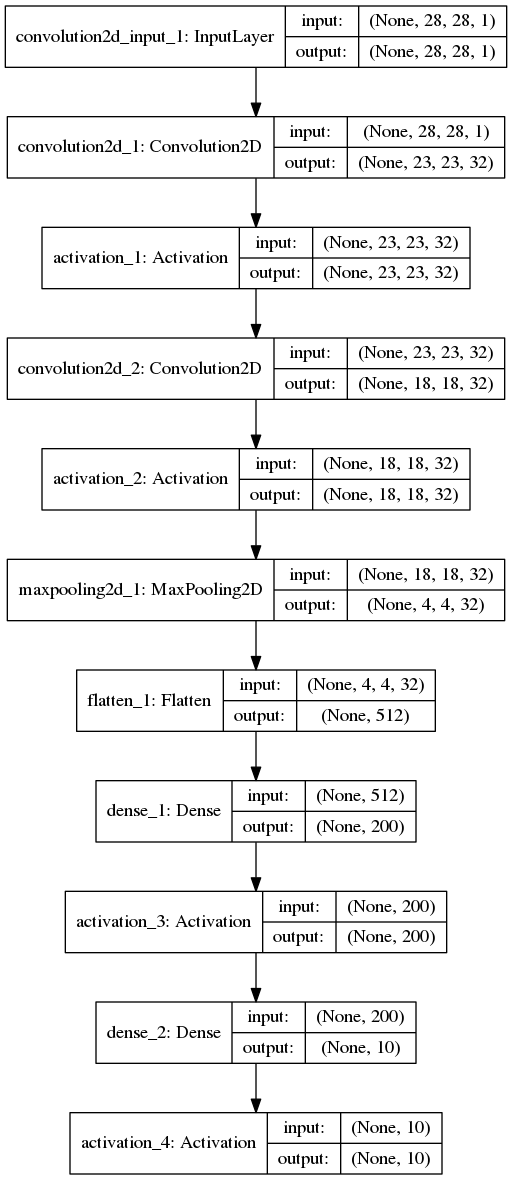
\includegraphics[width=.4\linewidth]{images/resultados/default/model}
	\end{minipage}%
	\begin{minipage}{.33\textwidth}
		\centering
		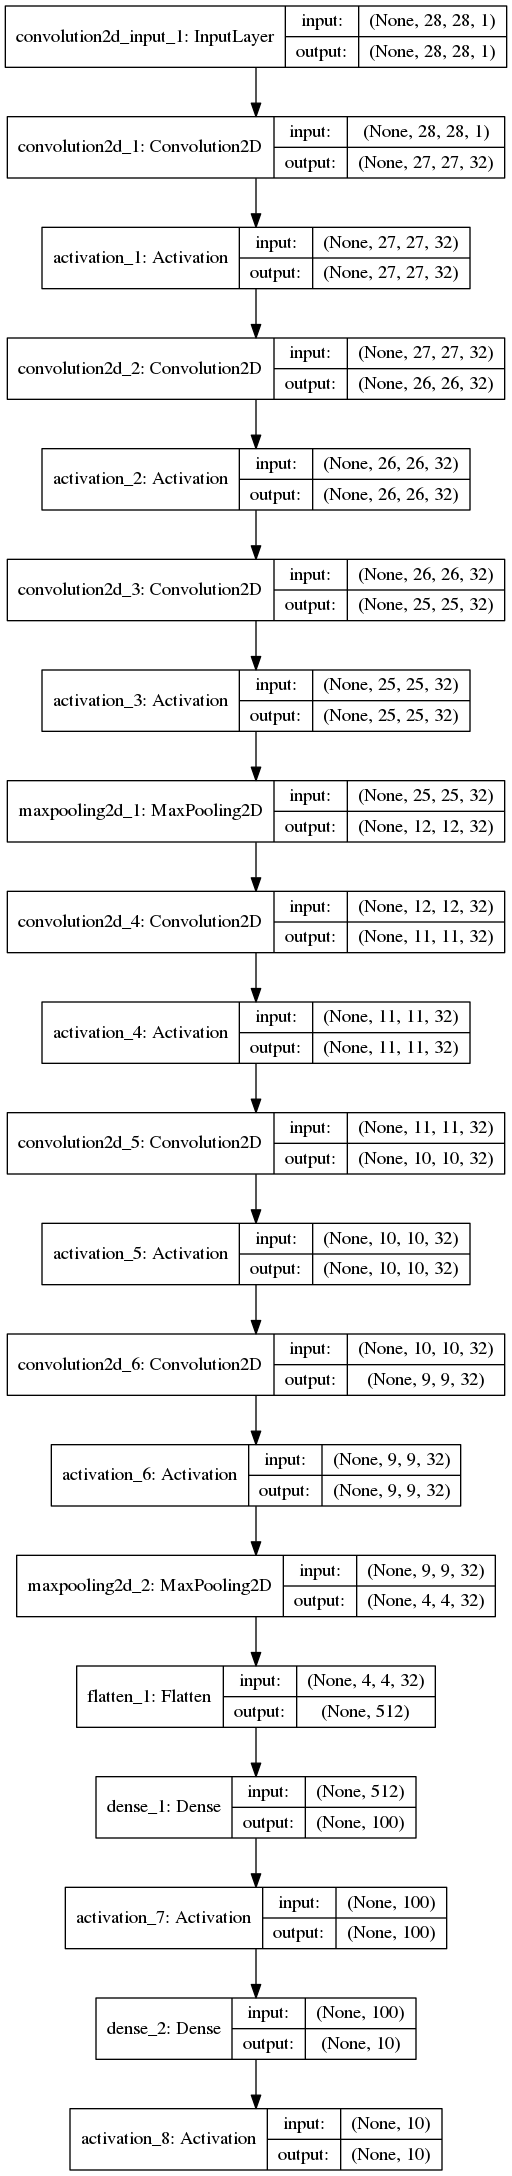
\includegraphics[width=.4\linewidth, height=.9\textheight]{images/resultados/network_1/model}
	\end{minipage}%
	\begin{minipage}{.34\textwidth}
	\centering
	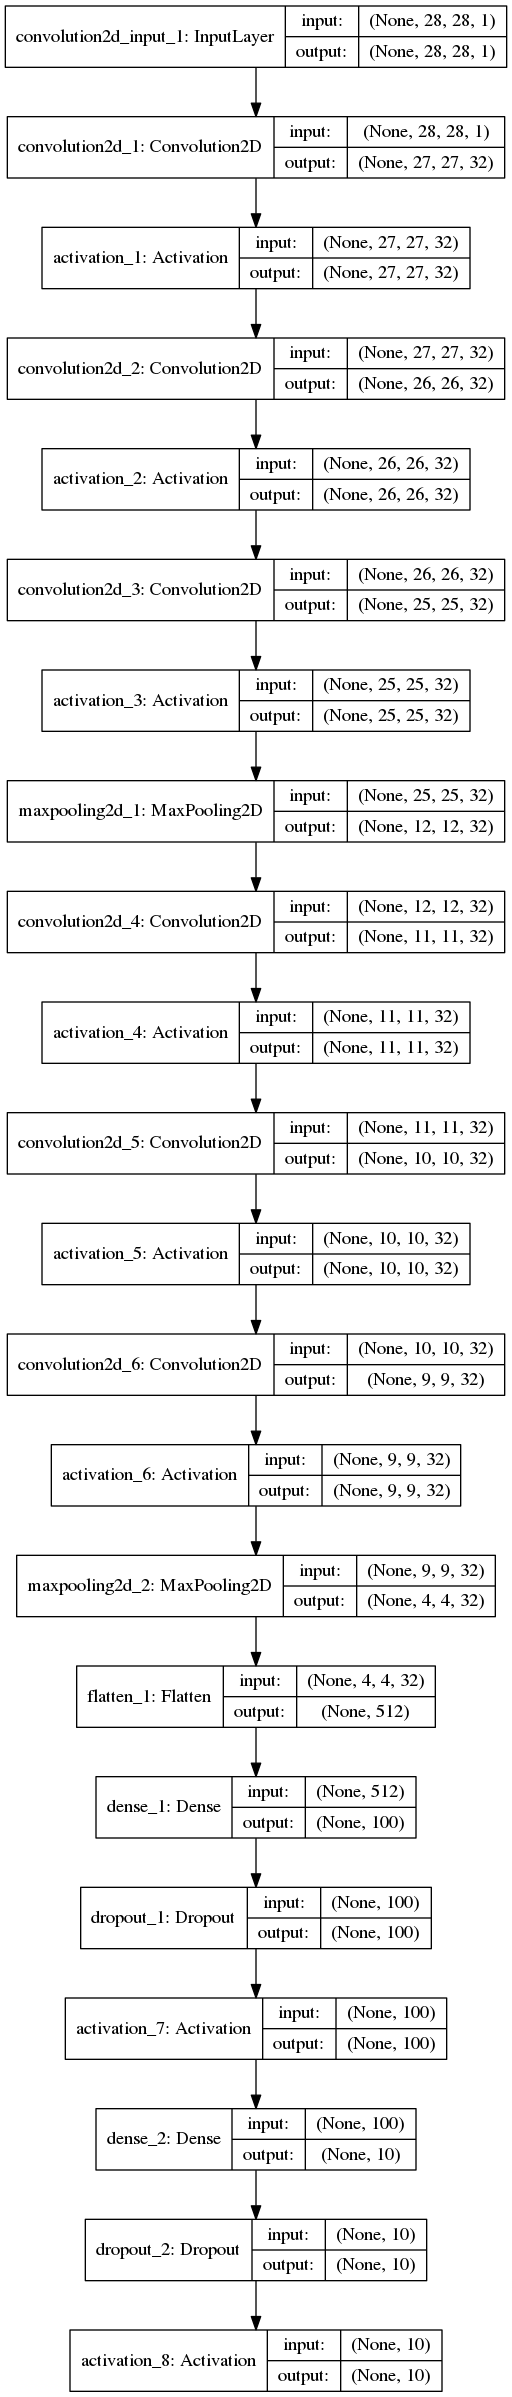
\includegraphics[width=.4\linewidth, height=.9\textheight]{images/resultados/network_2/model}
	\end{minipage}

\end{figure}

\end{frame}


\begin{frame}
	\frametitle{Camada de entrada}
	\centering
	MNIST DATASET
	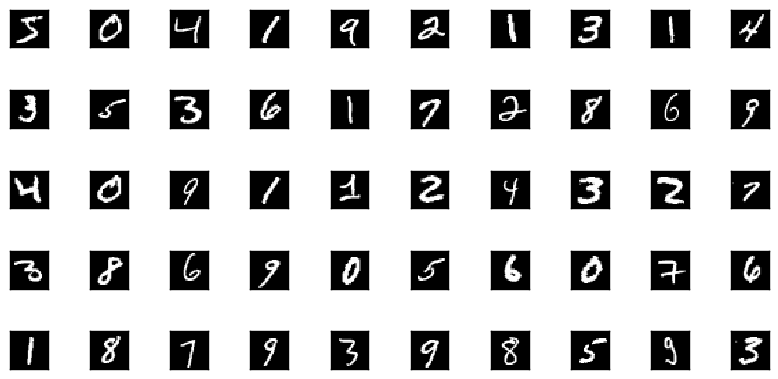
\includegraphics[width=.8\paperwidth]{images/fabio/inputs}
\end{frame}

\begin{frame}
	\frametitle{Aplicação da CNN}
	\centering
	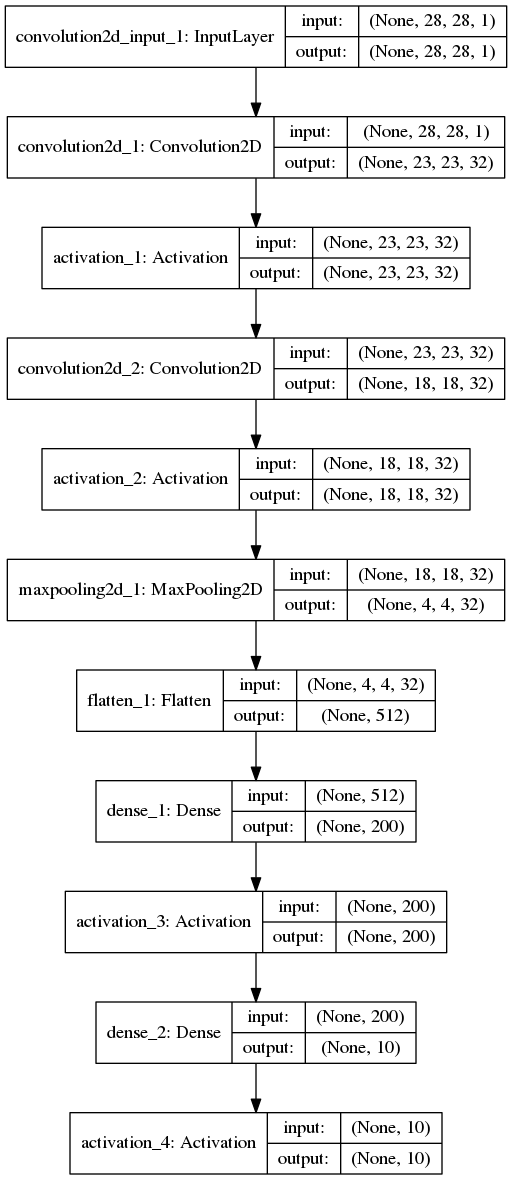
\includegraphics[height=.8\paperheight]{images/resultados/default/model}
\end{frame}

\begin{frame}
	\frametitle{Treinamento}
	\centering
%	\begin{minipage}{.5\textwidth}
		\centering
		\par Treinamento
		\begin{itemize}
			\item Épocas = 10
			\item Itens = 60000
			\item Tempo = 30 ~ 40 minutos
		\end{itemize}		
%	\end{minipage}%
%	\begin{minipage}{.5\textwidth}
	\centering
	\par Teste
	\begin{itemize}
		\item Itens = 10000
	\end{itemize}		
	\centering
	\par Resultado na base de teste
	\begin{itemize}
		\item 98.02\%
	\end{itemize}
%\end{minipage}%

\end{frame}

\begin{frame}
	\frametitle{Convolução - 1}
	\centering
	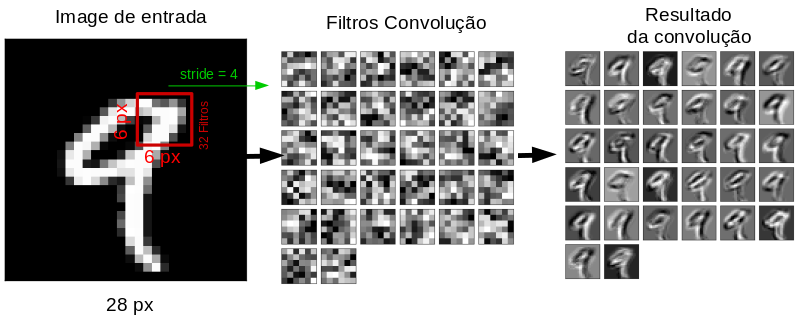
\includegraphics[width=.8\paperwidth]{images/fabio/conv_1}
\end{frame}

\begin{frame}
	\frametitle{Ativação - 1}
	\centering
	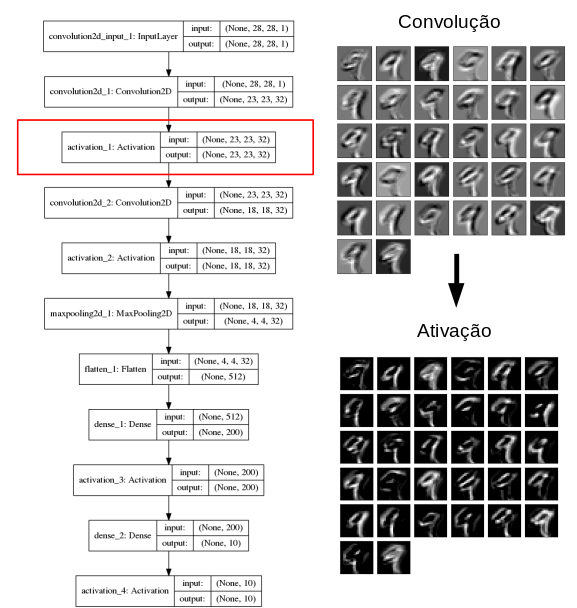
\includegraphics[height=.8\paperheight]{images/fabio/ativ_1}
\end{frame}

\begin{frame}
	\frametitle{Convolução - 2}
	\centering
	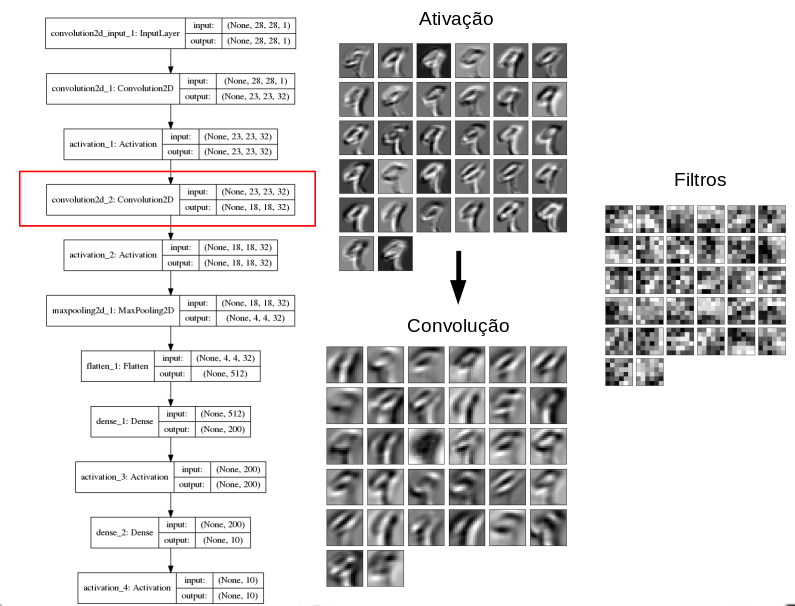
\includegraphics[width=.8\paperwidth]{images/fabio/conv_2}
\end{frame}

\begin{frame}
	\frametitle{Ativação - 2}
	\centering
	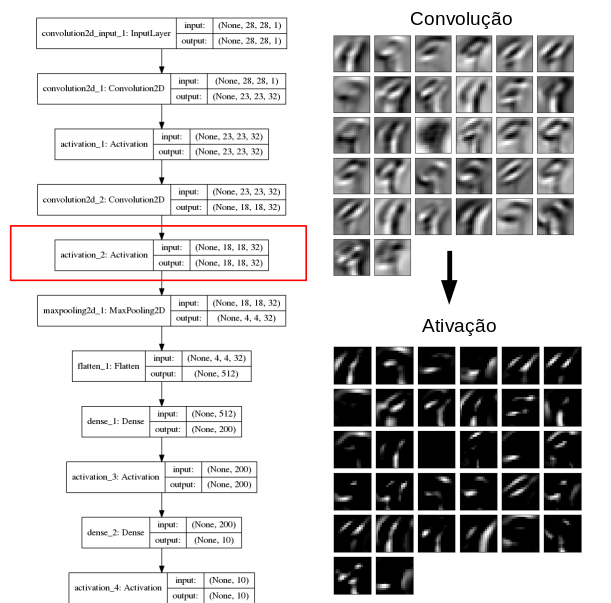
\includegraphics[height=.8\paperheight]{images/fabio/ativ_2}
\end{frame}

\begin{frame}
	\frametitle{Pooling}
	\centering
	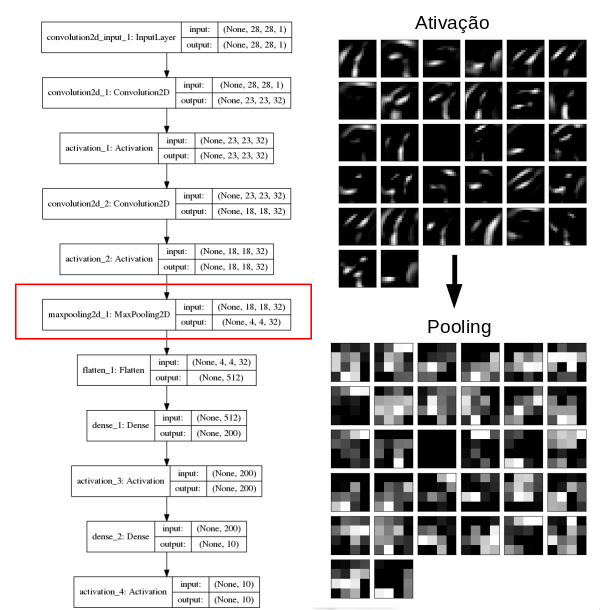
\includegraphics[height=.8\paperheight]{images/fabio/pooling_1}
\end{frame}

\begin{frame}
	\frametitle{Flatten ( N * 2D -> 1D)}
	\centering
	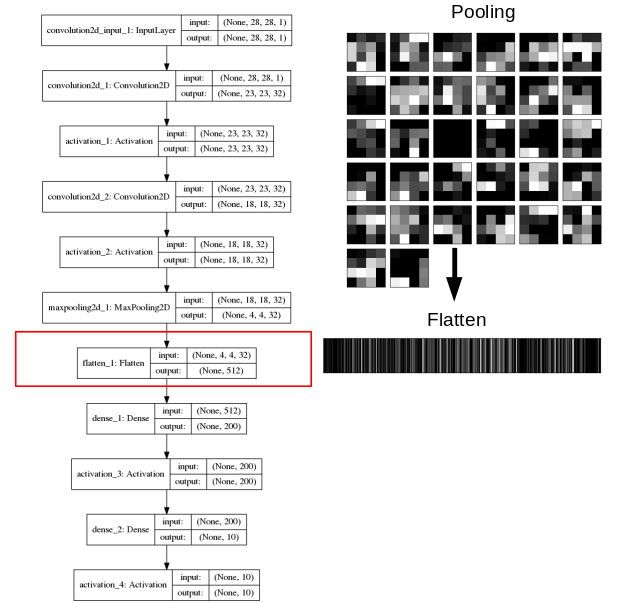
\includegraphics[height=.8\paperheight]{images/fabio/flatten_1}
\end{frame}


\begin{frame}
	\frametitle{Dense - 1}
	\centering
	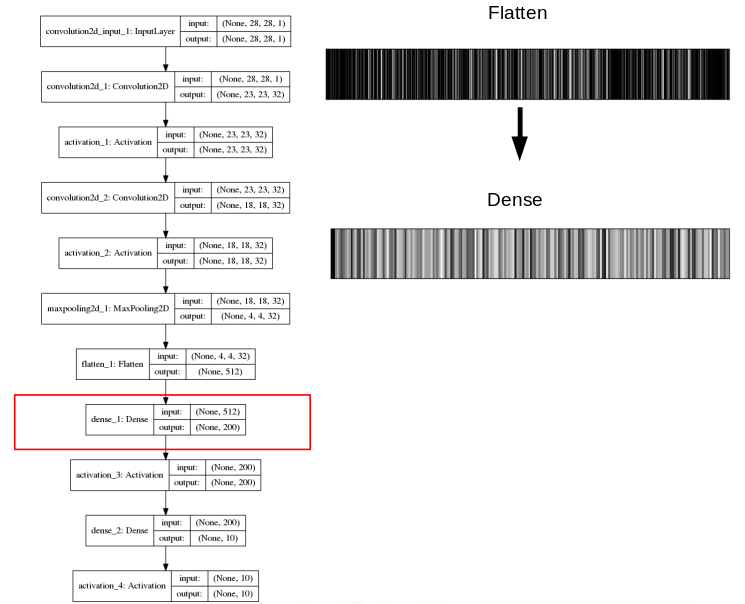
\includegraphics[height=.8\paperheight]{images/fabio/dense1}
\end{frame}

\begin{frame}
	\frametitle{Ativação - 3}
	\centering
	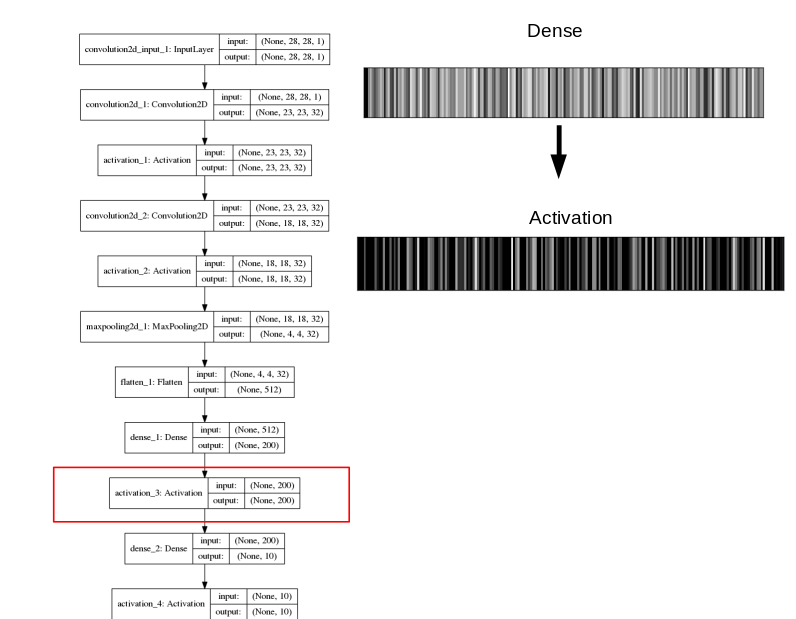
\includegraphics[height=.8\paperheight]{images/fabio/ativ_3}
\end{frame}

\begin{frame}
	\frametitle{Dense - 2}
	\centering
	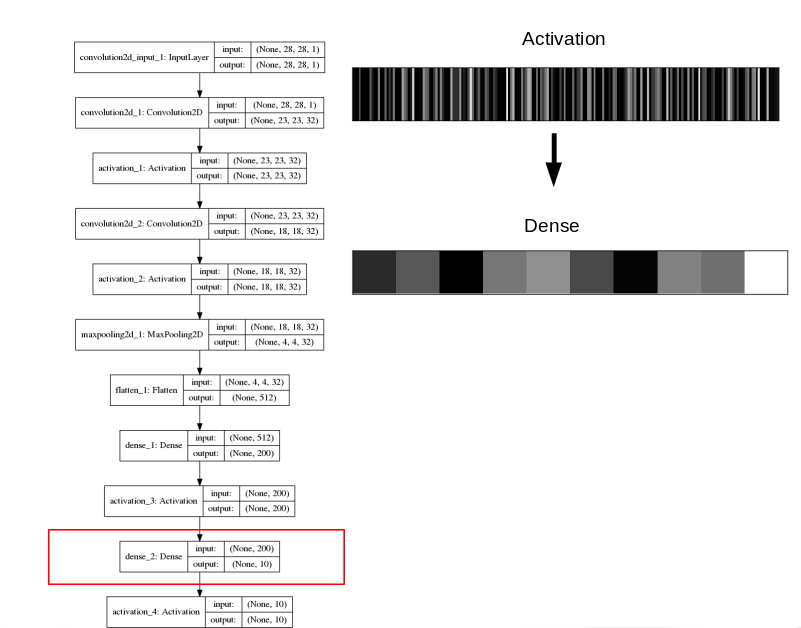
\includegraphics[height=.8\paperheight]{images/fabio/dense2}
\end{frame}

\begin{frame}
	\frametitle{Ativação - 4}
	\centering
	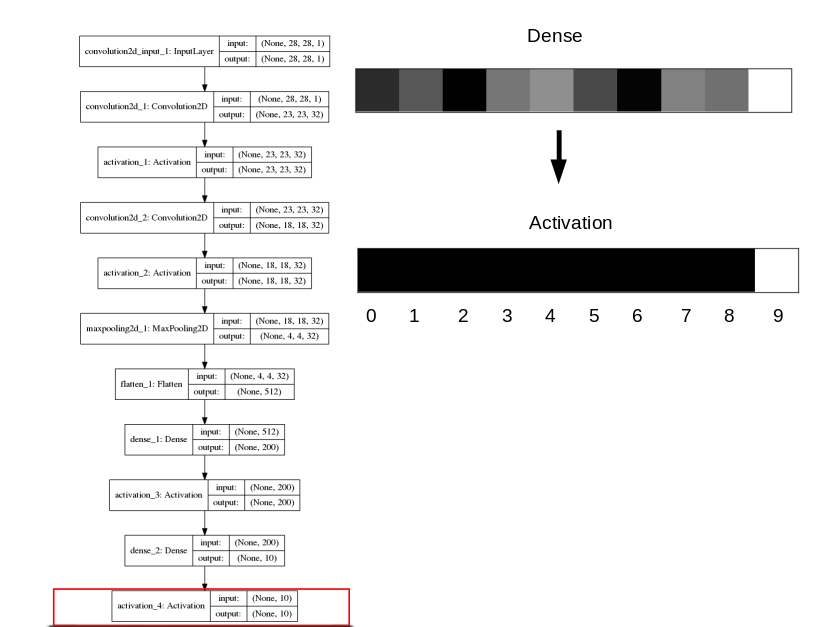
\includegraphics[height=.8\paperheight]{images/fabio/ativ_4}
\end{frame}


\begin{frame}
	\frametitle{Resultados das demais redes testadas - 1 }
	\centering
	\par Precisão na base de treino: 98.94\%
	\par Precisão na base de teste: 98.89\%
	\par 3 conv + 1 pooling + 3 conv + 1 pooling + 2 FC 
	\\
	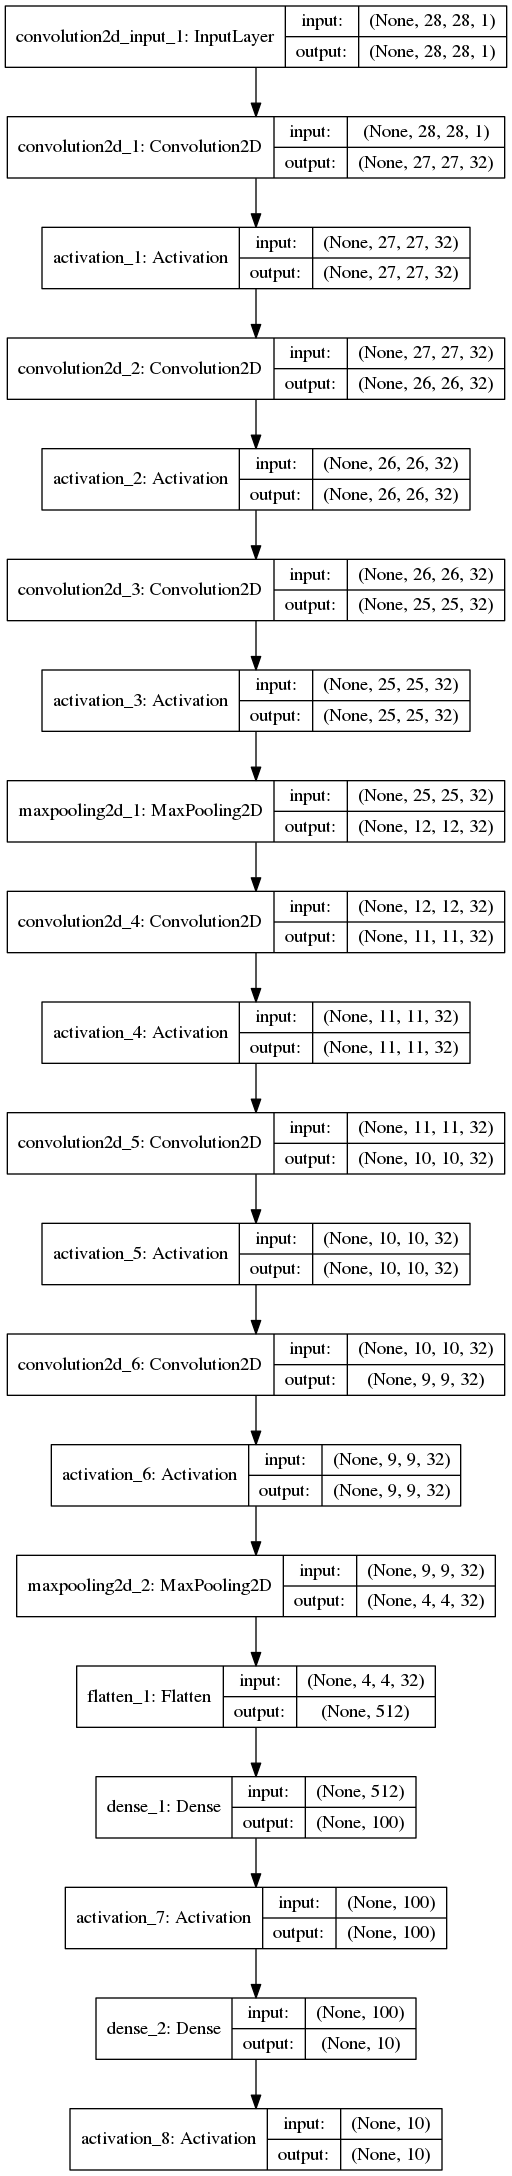
\includegraphics[height=.7\paperheight]{images/resultados/network_1/model}
\end{frame}

\begin{frame}
	\frametitle{Resultados das demais redes testadas - 2 }
	\centering
	\par Precisão na base de treino: 98.94\%
	\par Precisão na base de teste: 99.06\%
	\par 3 conv + 1 pooling + 3 conv + 1 pooling + 2 FC \(com dropout\)
	\\
	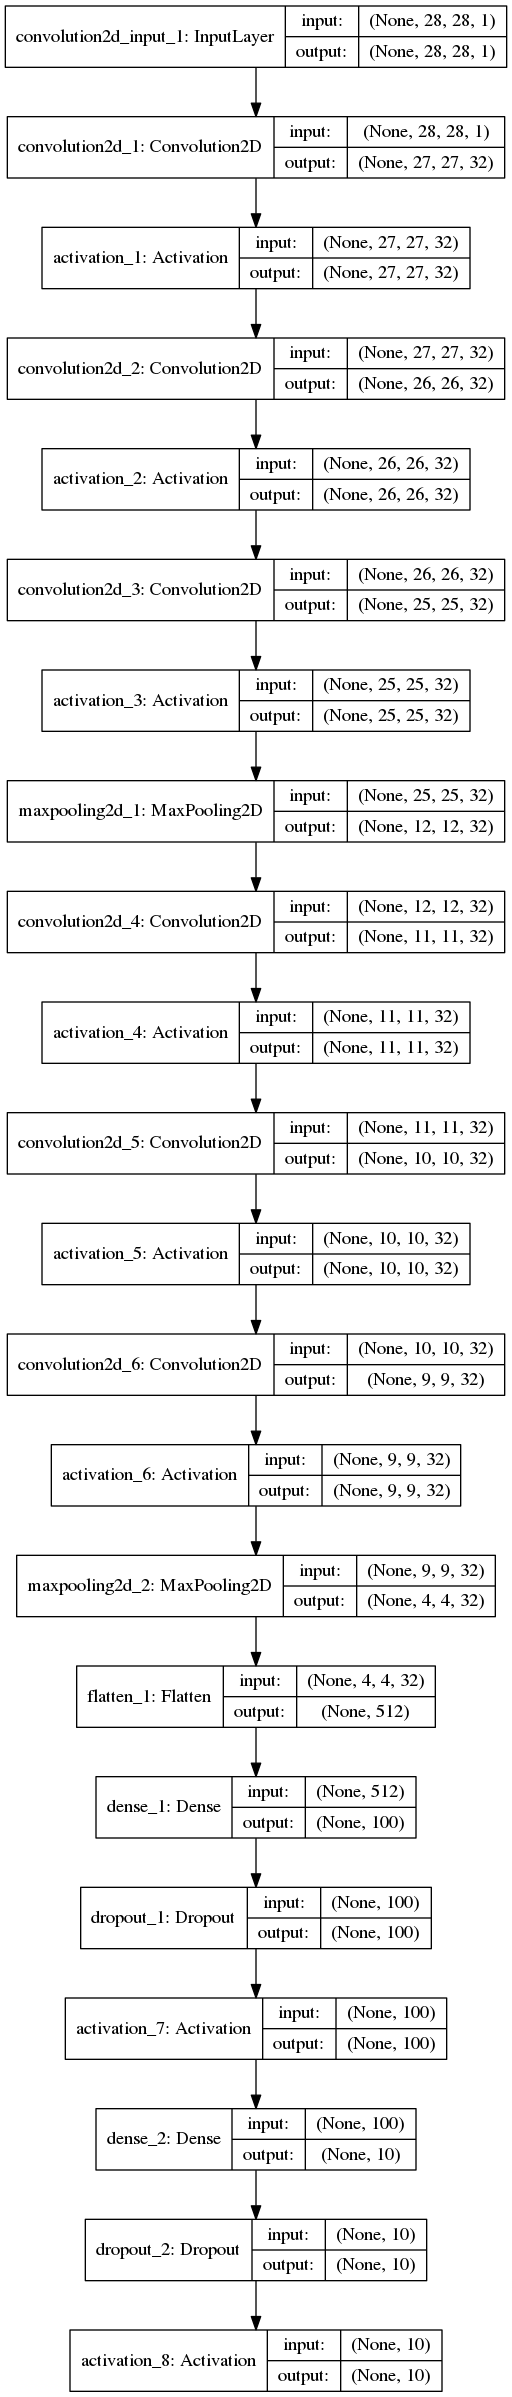
\includegraphics[height=.7\paperheight]{images/resultados/network_2/model}
\end{frame}

\begin{frame}
	\frametitle{MLP \& CNN}
	\centering
	\begin{itemize}
		\item CNN é uma extensão do conceito da MLP
		\item Convoluções e Pooling ajudam a diminuir rapidamente o número de variáveis do sistema
		\item Próprio para o processamento de imagens e vídeos		
	\end{itemize}
\end{frame}

% -------------------------------------------------
% end{fabio}
% -------------------------------------------------
\end{document}